\chapter{Results of Uncertainty Analysis}
\label{appendix-uncertainty}

A summary of the results of each model variation and method pairing was included in the main text of this study. This appendix will include a more detailed look at the individual results of the uncertainty analysis, for reference. To accomplish this, the data gathered will be visualized as pair plots, which visualize the relationships between each pair of outcome variables. These plots can reveal relationships between outcomes of interest that are useful in analysis and decision making. 

\section{Intertemporal Results}

\begin{figure}[h]
    \centering
    
    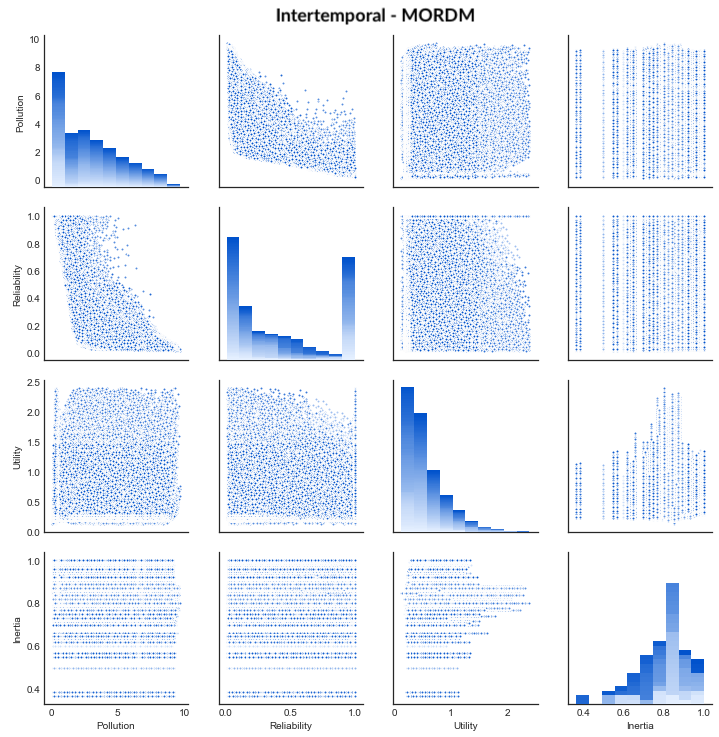
\includegraphics[width=\textwidth]{appendices/uncertainty_analysis/mordm_intertemporal}
    \caption[Intertemporal + MORDM pair plot]{Pair-plot showing the results of uncertainty analysis for a MORDM-based analysis of the intertemporal lake problem.}
    \label{fig:pairplot-mordm-inter}
\end{figure}

Very few relationships of any significance are revealed in \cref{fig:pairplot-mordm-inter}, graphing the results of the intertemporal and MORDM pairing. The plot does show a negative correlation between pollution level and reliability. Given that reliability refers to the ability of the policy to maintain low levels of pollution, it follows quite easily that higher pollution levels is paired with lower policy reliability. That same relationship is seen in \cref{fig:pairplot-multi-inter}, the plot of the results of the intertemporal and multi-scenairo MORDM pairing and even more significantly in \cref{fig:pairplot-moro-inter}, the results of the intertemporal and MORO pairing. 

\begin{figure}[h!]
    \centering
    
    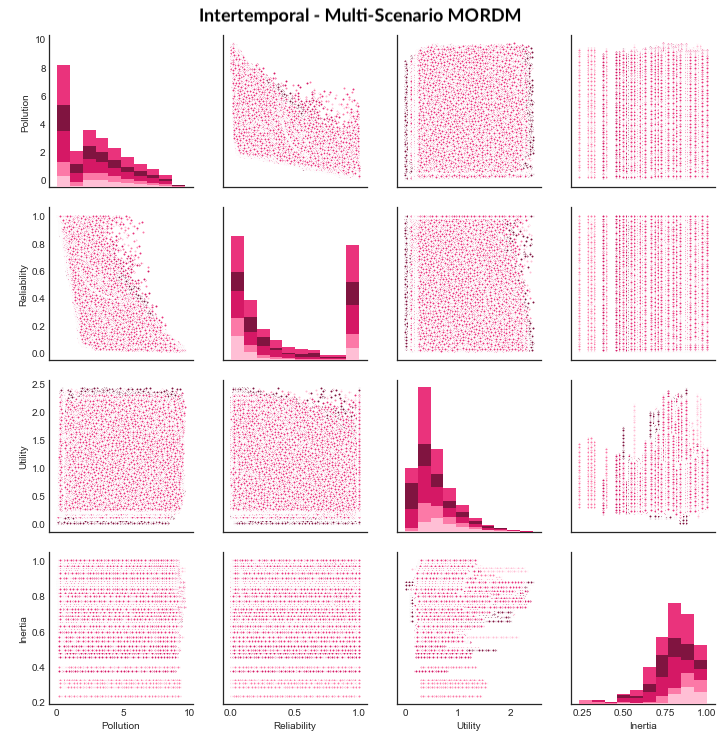
\includegraphics[width=\textwidth]{appendices/uncertainty_analysis/multi_intertemporal}
    \caption[Intertemporal + multi-scenario MORDM pair plot]{Pair-plot showing the results of uncertainty analysis for a multi-scenario MORDM-based analysis of the intertemporal lake problem.}
    \label{fig:pairplot-multi-inter}
\end{figure}

\cref{fig:pairplot-moro-inter}, the results of the intertemporal and MORO pairing, also reveal interesting behavior with respect to the inertia of identified policies, where only very low and very high values for inertia are reported. This behavior was investigated in more detail in \cref{chapter-comparison}. 

\begin{figure}[H]
    \centering
    
    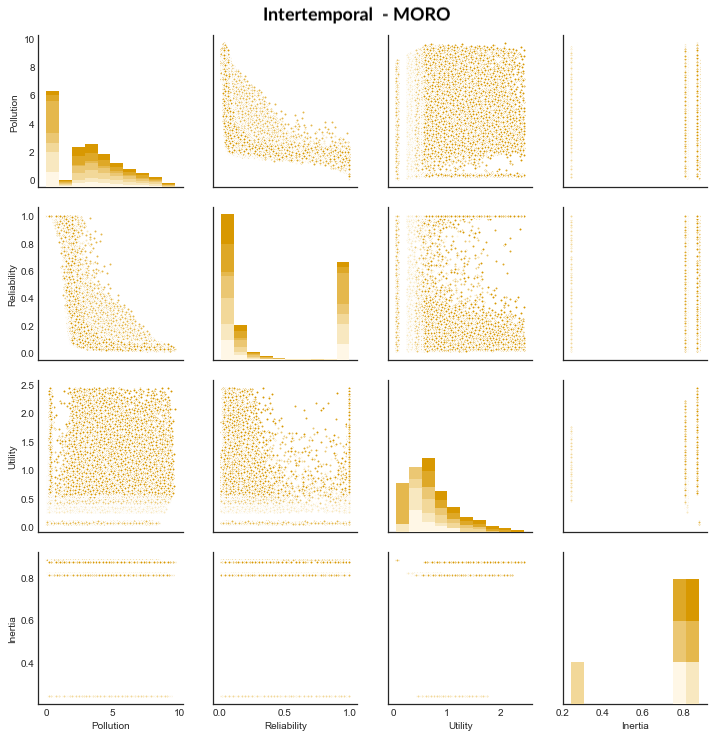
\includegraphics[width=\textwidth]{appendices/uncertainty_analysis/moro_intertemporal}
    \caption[Intertemporal + MORO pair plot]{Pair-plot showing the results of uncertainty analysis for a MORO-based analysis of the intertemporal lake problem.}
    \label{fig:pairplot-moro-inter}
\end{figure}

\newpage

\section{Planned Adaptive DPS Results} \label{pairplots-planned}
The relationship between pollution and reliability continues across all methods in the case of the planned adaptive DPS variation, though that relationship does not appear as strong in the multi-scenario MORDM case as it is for the other two methods. Both the multi-scenario MORDM and MORO methods seem to report a slight positive relationship between inertia and pollution level, where higher pollution levels lead to higher policy inertia. Given that policy inertia indicates that the amount of pollution released in each time step does not change significantly, it is not surprising that more constant rates of release may lead to higher levels of pollution in the lake. Interestingly, the opposite relationship is seen in the MORDM analysis of the planned adaptive DPS model, where higher levels of inertia lead to lower pollution levels. It is unclear given these pair plots why the relationship between the two outcomes of interest is different in the MORDM case than with the other two methods. 

\begin{figure}[H]
    \centering
    
    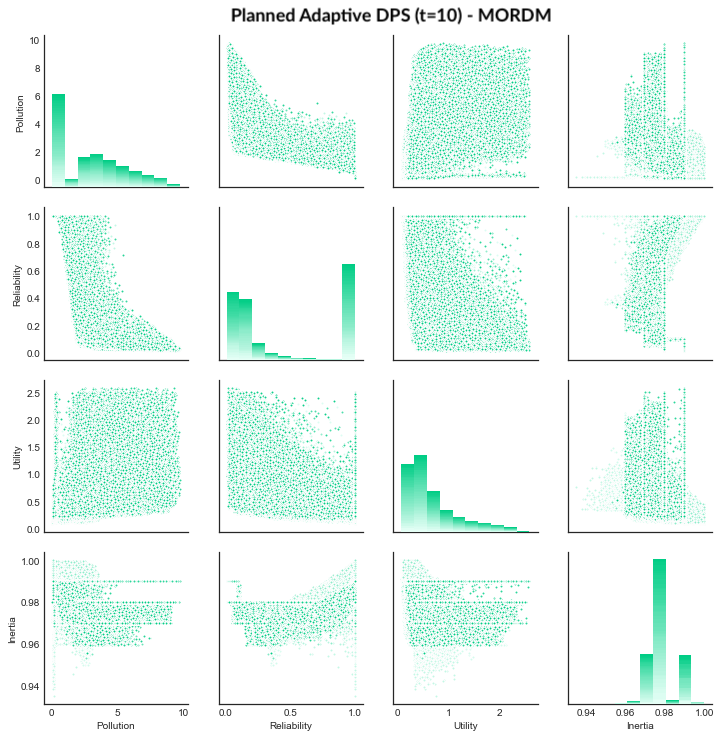
\includegraphics[width=\textwidth]{appendices/uncertainty_analysis/mordm_planned}
    \caption[Planned adaptive DPS + MORDM pair plot]{Pair-plot showing the results of uncertainty analysis for a MORDM-based analysis of the planned adaptive DPS lake problem.}
    \label{fig:pairplot-mordm-planned}
\end{figure}

\begin{figure}[H]
    \centering
    
    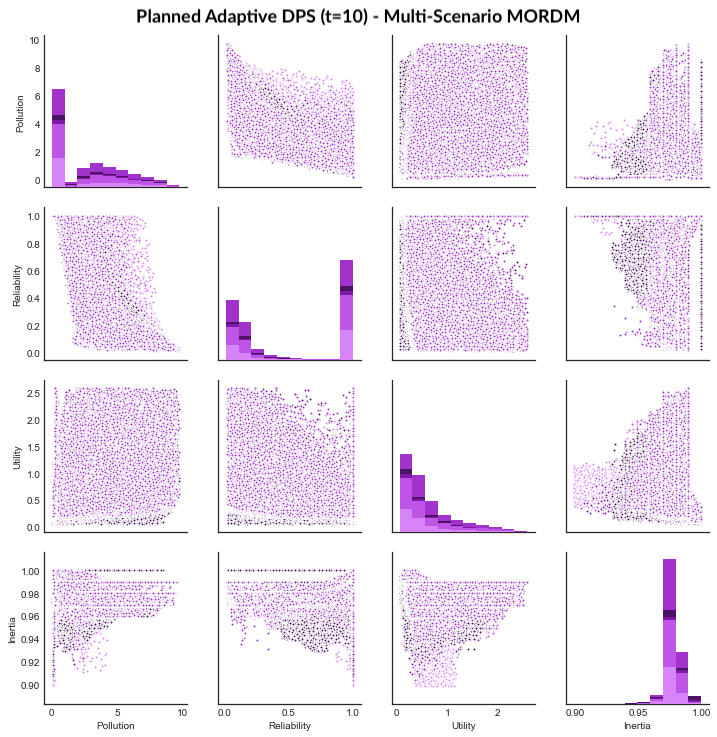
\includegraphics[width=\textwidth]{appendices/uncertainty_analysis/multi_planned}
    \caption[Planned adaptive DPS + multi-scenario MORDM pair plot]{Pair-plot showing the results of uncertainty analysis for a multi-scenario MORDM-based analysis of the planned adaptive DPS lake problem.}
    \label{fig:pairplot-multi-planned}
\end{figure}

\begin{figure}[H]
    \centering
    
    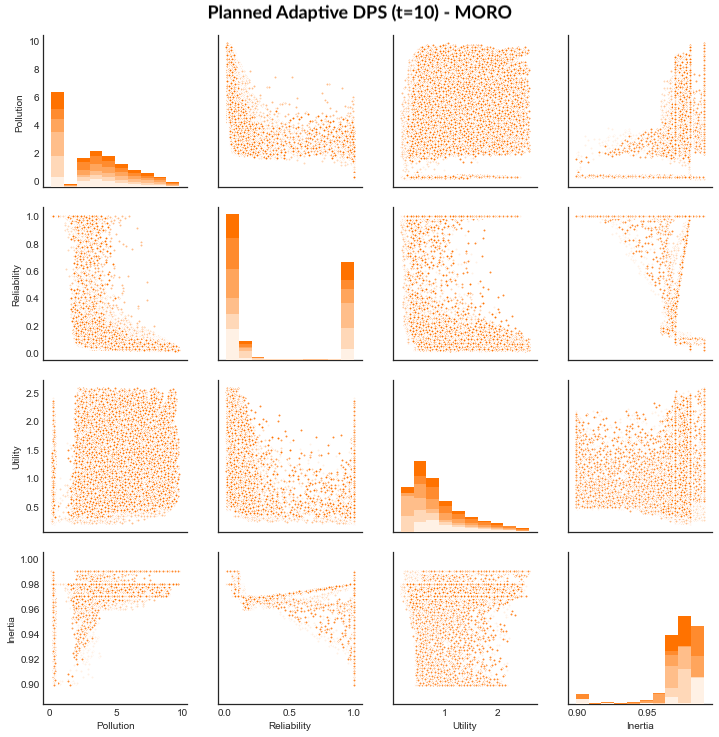
\includegraphics[width=\textwidth]{appendices/uncertainty_analysis/moro_planned}
    \caption[Planned adaptive DPS + MORO pair plot]{Pair-plot showing the results of uncertainty analysis for a MORO-based analysis of the planned adaptive DPS lake problem.}
    \label{fig:pairplot-moro-planned}
\end{figure}

\newpage

\section{Direct Policy Search Results}

The final set of pair plots involve the DPS model variation. The negative relationship between pollution level and reliability is not as strong for all three methods using the DPS model variation, as compared to the other two variations. There exists, however, a strong positive correlation between pollution and inertia for all three methods similar to what is seen and discussed in \cref{pairplots-planned}. An even stronger negative relationship between inertia and reliability is seen across all three methods as well, where higher levels of inertia lead to lower reliability. This relationship matches the relationships between pollution and reliability, and between inertia and reliability described previously. Higher levels of inertia mean the pollution level is not updated as frequently, which can make it more likely for the pollution level in the lake to rise and therefore reliability of that policy to decline.

\begin{figure}[H]
    \centering
    
    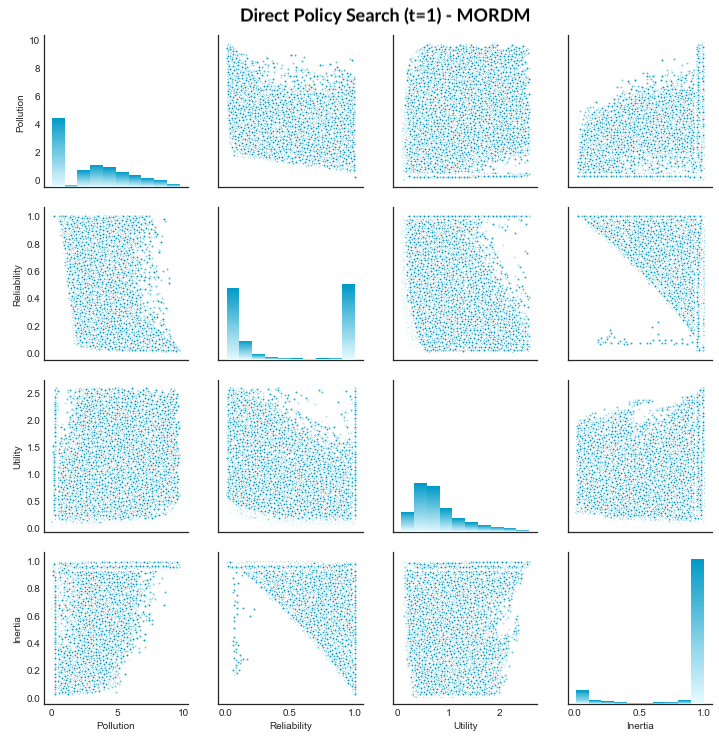
\includegraphics[width=\textwidth]{appendices/uncertainty_analysis/mordm_dps}
    \caption[DPS + MORDM pair plot]{Pair-plot showing the results of uncertainty analysis for a MORDM-based analysis of the DPS lake problem.}
    \label{fig:pairplot-mordm-dps}
\end{figure}

\begin{figure}[H]
    \centering
    
    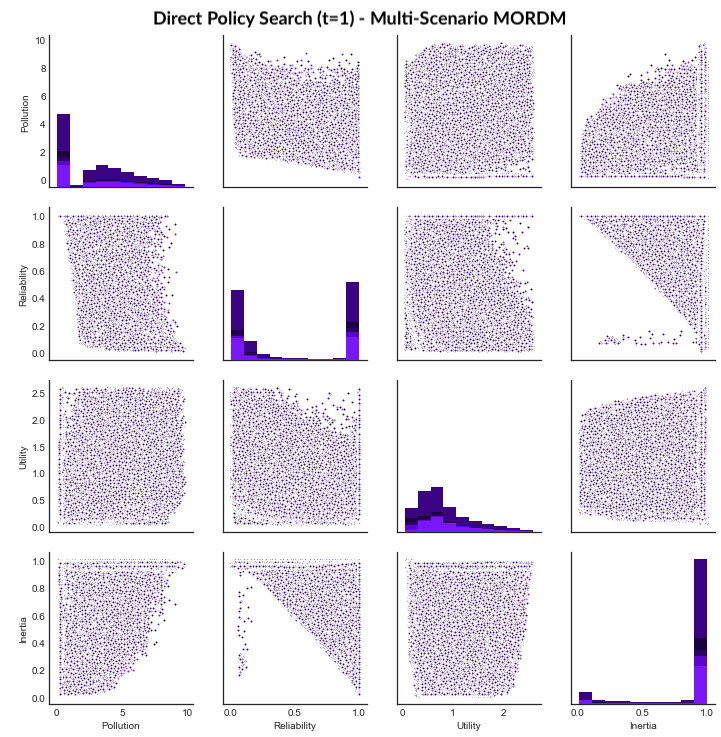
\includegraphics[width=\textwidth]{appendices/uncertainty_analysis/multi_dps}
    \caption[DPS + multi-scenario MORDM pair plot]{Pair-plot showing the results of uncertainty analysis for a multi-scenario MORDM-based analysis of the DPS lake problem.}
    \label{fig:pairplot-multi-dps}
\end{figure}

\begin{figure}[H]
    \centering
    
    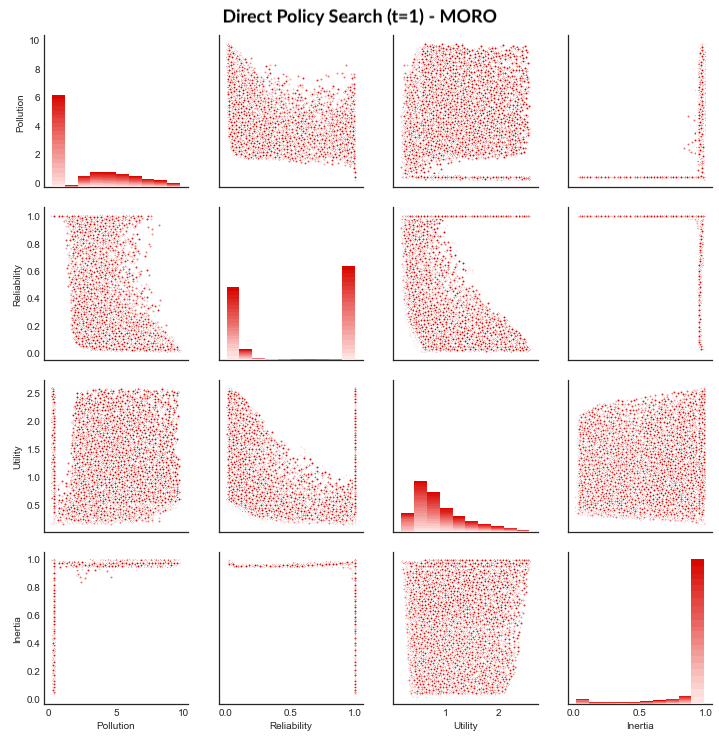
\includegraphics[width=\textwidth]{appendices/uncertainty_analysis/moro_dps}
    \caption[DPS + MORO pair plot]{Pair-plot showing the results of uncertainty analysis for a MORO-based analysis of the DPS lake problem.}
    \label{fig:pairplot-moro-dps}
\end{figure}